\chapter{新闻广播故事分割建模}
本章主要研究在广播新闻的语音识别结果上的故事分割,这属于一个自然语言处理的任务。在建模自然语言处理任务时,根据任务的不同,对于数据的可交换性假设也不同,如在文本分类的任务中,通常假设单个文本段内的单词是可交换的,即没有顺序关系,而在分词的任务中,则假设字之间是有顺序关系的,从而对不同的任务建立的模型区别很大。而广播新闻故事分割任务,则介于二者之间,通常先将新闻先切分为一些文本块,在建模时,假设文本块内部是可交换的,而文本块之间是不可交换的。

\section{故事分割任务分析}
故事分割就是将一段文本流分割成一系列段落,使得同一段落内有一定的相关性,而不同段落间有一定的差异性。本文主要研究广播新闻故事分割,此处文本流对应了未分割的完整新闻,段落对应了每个独立新闻故事(story),我们的任务是得到这些独立的新闻故事,即确定故事的边界。

在故事分割建模中,一般先根据文本的标点信息将文本流切割为一些子块(block)~\footnote{
在新闻广播的分割中,由于数据是语音识别的结果,无法获取标点信息,所以本文利用语音激活检测(Voice Activity Detection,VAD)的结果来切割子块。},这里假设每个子块内的单词是可交换的,所以可以用一个词频向量来表示。模型中将每个子块作为一个观察样本,然后在其组成的数据流上进行分割任务。

本文用$x_i$表示第$i$个样本,故事记作${S}_j = \{x_k|x_k\text{属于第}j\text{个故事}\},j \in {1...J}$,其中J是整段新闻中的故事个数。

\section{基线系统}
\subsection{TextTiling}

通常,同一个故事内部用词相似,比如篮球新闻播报过程中,可能反复提及三分、助攻等词,而政治新闻中则重复出现重申、强调等词,所以可以合理的假设同一个故事$S_j$内部的样本在词频上具有较大相似性,而不同故事$S_j$和$S_i$的样本之间具有较大差异性。所以一个直观的分割方法就是定义一个度量相似性的函数,然后计算相邻的$x_i$和$x_{i+1}$之间的相似性,如果其低于某个阈值,就认为其之间差异性过大,即分属两个不同的故事。

然而这种简单的方法容易被一些噪声干扰,为了增加鲁棒性,hearst引入了深度值的概念,即在相似度曲线上,只将处于波谷的点作为边界候选点,然后计算该点到左右两个相邻的波峰点的下降值之和,称之为深度值,如果某点的深度值大于阈值,就认为该点是故事边界。这一方法称为TextTiling方法\cite{HEA:97}。

\subsection{隐语义分析}
一般的相似度度量采用词频分布上的余弦函数或者交叉熵,然而词频分布向量的维度很大,这种度量方法的结果不佳。如果认为每个故事都是由一系列主题混合而成,即不同故事间共享主题,但是每个故事在不同主题上的权重不同,则可以用主题成分上的权重作为特征。这正是\ref{subsec:lda}小节中的LDA模型。如果不为混合参数加一个先验,则得到一个非贝叶斯模型,称为PLSA模型。

当得到主题成分时,就可以在$x_i$上计算其对应的主题分布,如果使用主题分布作为$x_i$的特征,这样就将一个高维的表示变为一个K维的表示。

然而这一方法是有监督的,因为需要提供一份已标注好故事边界且和待分割的文本领域相同的语料来训练出主题成分,不然共享相同的主题这一假设就不成立。~\footnote{LDA经常用于无监督建模,因为对于LDA而言语料本身已经是划分好的,这里说的有监督,是指整个系统}

\subsection{全局最优算法}
在textiling中,根据相邻点的相似度来寻找边界,这是一种局部的贪心算法。考虑建立一个全局上最优的算法,即对于某种能够衡量段内相似度的度量函数$sim$,期望得到一个划分${\bm \pi}$,使得全局的得分最大:
\begin{equation}
{\bm \pi} = argmax_{\bm \pi}{\sum_{j=1}^{J}{sim({S}_j)}}
\end{equation} 

可以用下面的动态规划算法求得最优解:
\begin{equation}
\left\{
\begin{array}{l}
f(1) = sim({\bm x}_{1})\\
f(i) = \mathop{\max}\limits_{k\leq i}\{f(k-1)+sim({x}_{k\leftrightarrow i})\} \\
b(i) = \mathop{\arg\max}\limits_{k\leq i}{\{f(k-1)+sim({x}_{k\leftrightarrow i})\}}
\end{array}
\right.
\end{equation}
其中$f(i)$是从$x_1$到$x_i$间的样本对应的最优得分,$b(i)$记录最优边界的回溯值,${x}_{i\leftrightarrow j}$表示$x_i$到$x_j$间的所有样本。

然而,如果直接使用得分最高的划分,其分割结果和启发式的相似度测量函数的参数有关,如果参数设定不当,则效果较差,所以需要指定真实的分段个数n,此时动态算法要稍微复杂一些,变为:
\begin{equation}
\left\{
\begin{array}{ll}
f(1,i) = sim({\bm x}_{1 \leftrightarrow i})& \\
f(n,i) = \mathop{\max}\limits_{n\leq k\leq i}\{f(n,k-1)+sim({x}_{k\leftrightarrow i})\}  & 1 < n \leq N \\
b(n,i) = \mathop{\arg\max}\limits_{n\leq k\leq i}{\{f(n,k-1)+sim({x}_{k\leftrightarrow i})\}}  & 1 \leq n \leq N
\end{array}
\right.
\end{equation}
其中$f(n,i)$是从$x_1$到$x_i$间的样本分成n段对应的最优得分,$b(n,i)$记录最优边界的回溯值。

\section{贝叶斯概率模型}
本文考虑利用概率方法为故事分割任务建立一个概率模型。首先假设一段文本流由数个连续的故事组成,${x_k|x_k \in S_j}$之间是可以交换的,他们独立同分布于一个参数为$\theta_j$的离散分布,而$x_m \in S_a$和$x_n \in S_b$($a \neq b$)之间是不可交换的。另外,$S_i$和$S_j$之间是可交换的,则$\theta_j$是独立同分布于一个概率分布的。取一个参数为$\lambda_0$的Dirichlet分布作为${\bm \theta}$的共轭先验,并设$x_i$对应的故事为$z_i$,则对于某个划分$Z$模型的似然为:
\begin{equation}
p(D|Z,\lambda_0) = \prod_{j=1}^J{p(S_j|\lambda_0)}  
\end{equation}
其中$S_j = \{x_t| t:z_t = j\}$,$p(S_j|\lambda_0)  = \int p(S_j|\theta_j)p(\theta_j|\lambda_0) d \theta_j $

由于$\{x_t| t:z_t = j\}$在观察到$\theta_j$的情况下是条件独立的,再根据Dirichlet分布的性质,可得整段文本的最大似然函数。
这一模型可以看做是Mincut框架的一种特例,和上述全局最优算法的区别在于其段内相似度的度量函数不是手工设定的,而是从概率建模中自然推导出来的,利用狄利克雷分布的共轭性质\cite{heinrich2005parameter},得:
\begin{equation}
\frac{\Gamma(V\lambda_0)\prod_v\Gamma(n_j^v+\lambda_0)}{\Gamma(n_j+V\lambda_0){\Gamma(\lambda_0)}^V}
\end{equation}
其中$\Gamma(x)$表示Gamma函数,$n_j^v$是第$j$个故事中单词v的个数,$n_j$是第$j$个故事中单词的个数,V是词表大小。

这一模型称为基于贝叶斯概率模型的分割方法(BayesSeg)。

\section{依赖于距离的中国餐馆过程}
\begin{figure}
  % Requires \usepackage{graphicx}
  \begin{center}
  \quad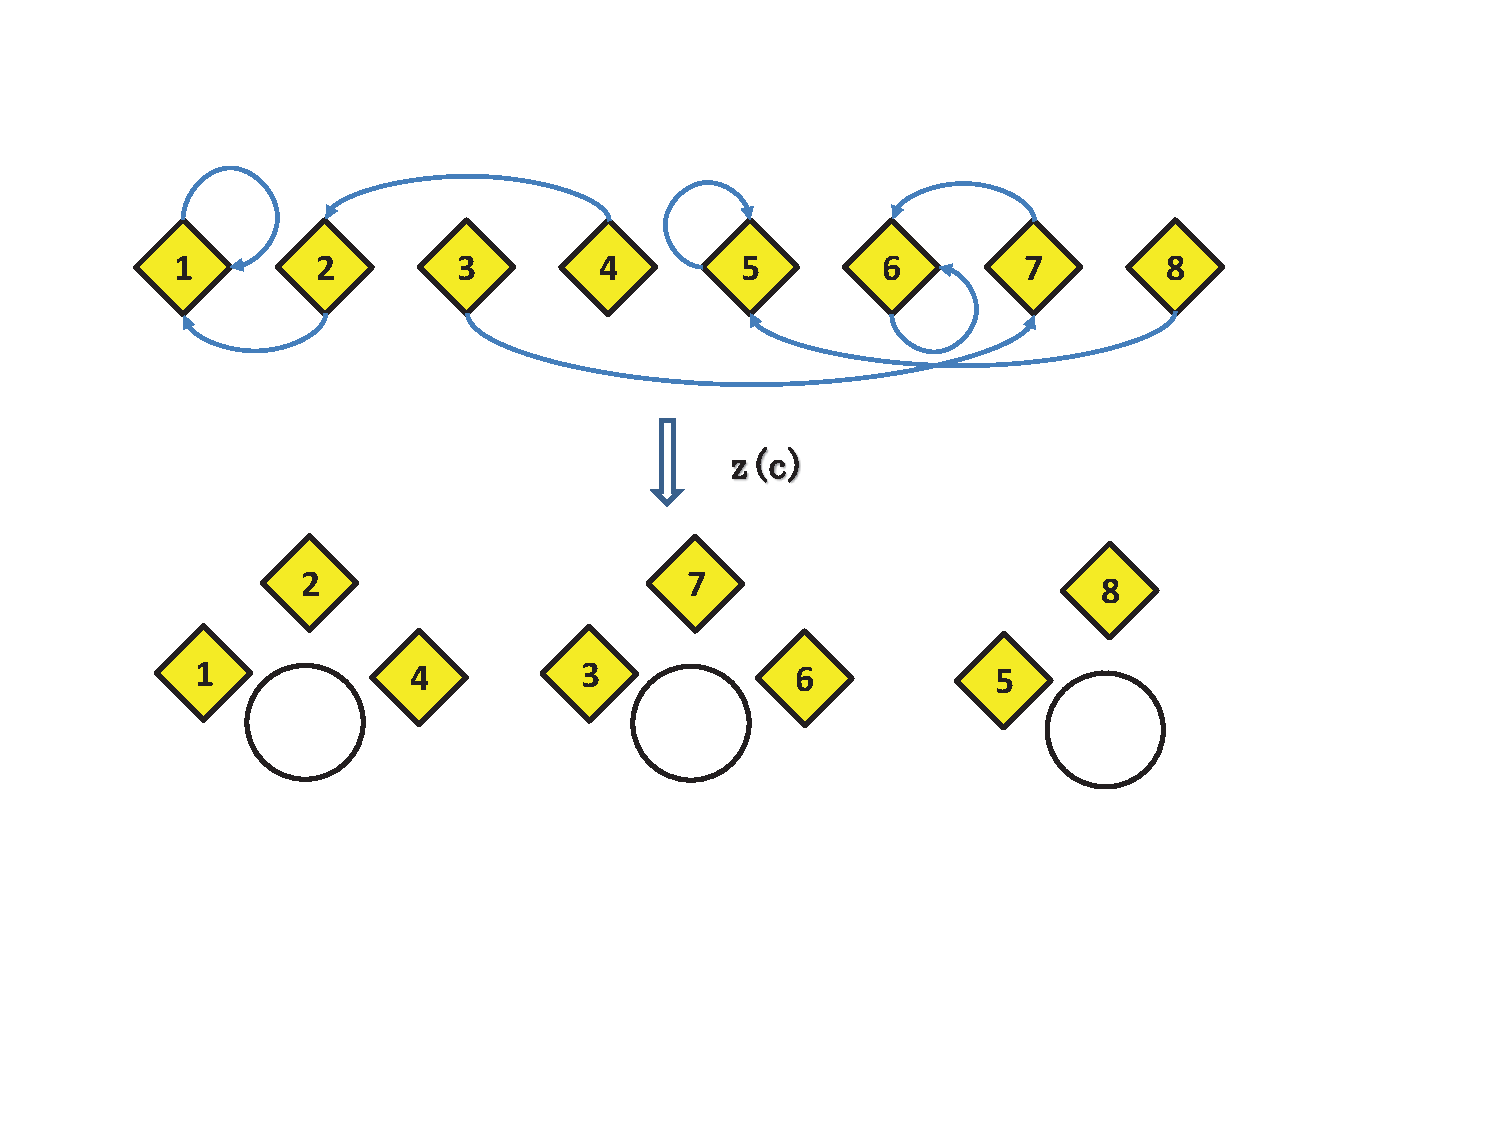
\includegraphics[width=0.8\textwidth]{c2z.eps}\\
  \end{center}
  \caption{依赖于距离的中国餐馆过程示意图.}
  \label{f:c2z}
\end{figure}
本文考虑为故事分割任务建立起非参数模型,克服一般分割方法需要给定切分个数的缺点。假设一段新闻是从如下过程中采样生成的:
首先,先采样出每个$x_i$的主题$z_i$。然后,对每个$z_i$,根据其对应的主题$\theta_{z_i}$,采样出$x_i$。但是这里并不能用中国餐馆过程作为z的先验,因为不同故事间的$x_i$和$x_j$是不能交换的。故必须寻找一种具有不可交换性的分布。这里考虑中国餐馆过程的一种变形,称为依赖于距离的中国餐馆过程(distance dependent CRP,dd-CRP)。这一过程并不直接建立起顾客到餐桌的划分,而是建立顾客和顾客之间的关系。如果引入一个顾客间的距离关系(比如越熟悉的顾客或者是拥有更多相同喜好的顾客之间距离就越小),认为对于一个新来的顾客,他会选择和与自己距离小的顾客坐在一起,用$c_i = j$表示$i$顾客选择了和顾客$j$坐在一起,这样通过$c_i,i = 1...N$也可以得到顾客到餐桌的一种划分$z_i,i = 1...N$。如图\ref{f:c2z}中所示,菱形代表顾客圆形代表桌子,顾客之间的箭头代表着顾客选择和谁坐在一起。在这个图中,第一个顾客$c_1$只能选择和自己坐在一起,顾客$c_2$选择和$c_1$ 坐在一起,顾客$c_4$选择和$c_2$坐在一起,没有其他的顾客和他们坐在一起,这样$c_1$ ,$c_2$, $c_4$坐在同一张座子上。这一过程的定义如下:
\begin{equation}
\label{eq2.2}
p(c_i=j|D,f,\alpha)\!\propto\!\left\{
\begin{array}{lll}
f(d_{ij}) \!\! & \text{if}\!\!\! & j \ne i \\
\alpha \!\! & \text{if}\!\!\! & j = i \\
\end{array}
\right.
\end{equation}

其中$D$是一个顾客之间距离测度的集合,$d_{ij}$是顾客$c_i$和$c_j$间的距离,$f(d)$是一个非增函数,因为顾客间的距离越大,坐在一起的概率就越小。
\begin{figure}
 \begin{center}
  \includegraphics[width=0.6\textwidth]{crpp.pdf}\\
  \end{center}
  \caption{CRP和dd-CRP的采样结果比较}\label{f:crpp}
\end{figure}

如果顾客之间的距离和他们的顺序是有关系的,那么这个模型具有不可交换性。本文
用这个过程作为故事分割中样本对应的$z_i$的先验分布。使用最简单的线性距离和0-1窗口函数,即对于$j < i$有$d_{ij} = i - j$,对$j > i$有$d_{ij} = \infty$,$f(d) = 1[d <= a]$,a是窗口大小,则根据生成过程可知,$x_i$的主题要么和前$a$个样本中的某一个一致,要么是一个新主题。这相当于为$z$增加了一个具有分割性质的先验。而CRP只能增加一个具有聚类性质却无分割性质的先验。图\ref{f:crpp}展示了两种过程的采样结果。可以看到,从CRP中的采样(图A和图B)的同一聚类点较分散,没有时间上的连续性。而dd-CRP中的采样(图C和图D)则是把相邻的点聚成一类,具有很好的分割性质。

\subsection{推断方法}
\begin{figure}
  \begin{center}
  \quad\includegraphics[angle=0,scale=0.6]{reassign.pdf}\\
  \end{center}
  \caption{dd-CRP单次gibbs采样时的情况}
  \label{fig:re}
\end{figure}
对于建立的上述模型,利用Gibbs采样的方法,根据每个$c_i$在其他变量上的条件概率依次进行采样。这里$G_0$选用Dirichlet分布,是$\phi_k$的共轭先验,从而每一步采样时可以将$\phi_k$积分掉,利用collapsed Gibbs采样提高收敛速度:
\begin{equation}p(c_i|c_{-i},x_{1:N},\theta,G_0)\propto p(c_i|\theta)p(x_{1:N}|z(c_{1:N}),G_0).\end{equation}
其中第一项是dd-CRP提供的先验,第二项是似然项。因为同一个餐桌上的观察值是独立同分布的,所以似然项是根据不同的餐桌因子化的,即:
\begin{equation}
p(x_{1:N}|z(c_{1:N}),G_0)=\prod_{k=1}^{|z(c)|}p(x_{z^{k}(c)}|G_0)\end{equation}
这里$|z(c)|$是桌子的总个数,$z^{k}(c)$是第$k$个桌子上所有的顾客对应的索引集合。

在采样$c_i$时,先移除掉从顾客$i$指出的箭头。根据$c_i$的重新取值对最终划分的影响,这里只有两类可能的情况,要么新的$c_i$将某两个桌子合并到一起,要么对于划分没有影响(图\ref{fig:re})。

对于第一种情况,令$l$ 和$m$代表被合并的两个桌子的标号,则关于$z^{l}$和$z^{m}$的两个似然因子项被合并为一个关于的$z^{l}(c)\cup z^{m}(c)$因子。而其他的因子不会改变。所以似然为:
\begin{equation}p(x_{z^{l}(c)\cup z^{m}(c)}|G_0)\prod_{k \ne m,l}p(x_{z^{k}(c)}|G_0)\end{equation}

对于第二种情况,所有的因子都不会改变,从而得到:
\begin{equation}
\begin{split}
&p(c_i|c_{-i},x_{1:N},\theta,G_0)\\
&\propto\left\{
\begin{array}{ll}
p(c_i|\theta)\Delta(x,z,G_0)  & c_i\ \text{joins} \ l\ \text{and} \ m\\
p(c_i|\theta)   & \text{otherwise} \\
\end{array}
\right.
\end{split}
\end{equation}
其中
\begin{equation}\Delta(x,z,G_0)=\frac{p(x_{z^{l}(c)\cup z^{m}(c)}|G_0)}{p(x_{z^{l}(c)}|G_0)p(x_{z^{m}(c)}|G_0)}\end{equation}

第$k$个因子项的似然为:
\begin{equation}
p(x_{z^{k}(c)}|G_0) = \int p(x_{z^{k}(c)}|\phi_k)p(\phi_k|G_0)d\phi_k
\end{equation}


\section{实验与分析}

\begin{table}
\begin{center}\small
\begin{tabular}{|l|l|l|l|}
\hline \bf 方法 & \bf F1 & \bf 方法 & \bf F1 \\ \hline
dd-CRP & 0.7357 & PLSA-DP-CE &  0.6815 \\ \hline
BayesSeg &  0.7137 & TextTiling & 0.5341 \\ \hline
\end{tabular}
\end{center}
\caption{实验结果}
\vspace{-2pt}\label{table:sg_result}
\end{table}
\subsection{实验设置}
本章的实验数据使用TDT2中英文广播新闻语料库\footnote{http://www.ldc.upenn.edu/Projects/TDT2}中的的VOA新闻,对本文提出的方法进行评估。语料来源于1998年2月至7月的美国之音英文广播新闻,共含111个新闻段,时长111小时。语料含有LVCSR识别文本及手工标注的过的真实边界。

\subparagraph{数据预处理}
对于所有的文本,使用Porter算法\cite{POR:09}对其进行处理,将单词进行stem化,并且去除掉停用词(stop word)。然后将文本切割成固定长度的文本块,且子块之间没有重合。对于每个文本块,将其转化为词频表示,作为模型的观察特征。
\begin{figure}\center
\vspace{10pt}
  % Requires \usepackage{graphicx}
  \quad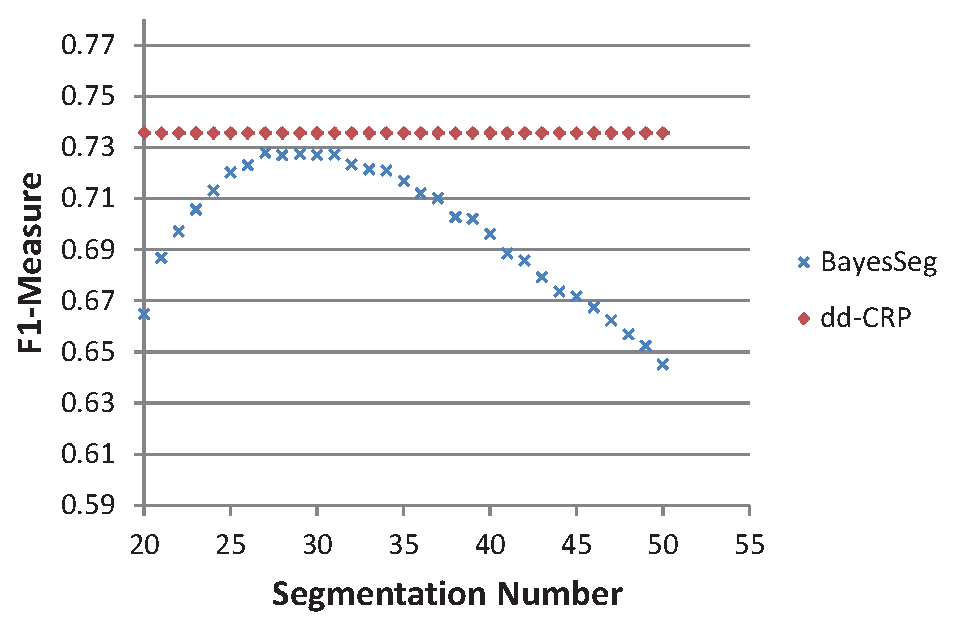
\includegraphics[width=0.6\textwidth]{comp.eps}\\
  \caption{BayeSeg受到分割个数的严重影响,如果设置不当,会导致结果下降很多,而dd-CRP则可以通过自动发现合适的分割个数来避免这一问题。}\label{fig:comp}
  \vspace{-12pt}
\end{figure}
\subparagraph{评价方法}
使用自然语言处理领域常用的F1测度作为实验的评价方法,其定义如下:
\begin{equation}
F1 = \frac{2*rec *pre}{rec+pre}
\end{equation}
其中,pre表示正确率(precision rate),即找到的正确边界数占找到的总边界数的比例。rec表示召回率(recall rate),即找到的正确边界数占真实故事边界数的比例。其定义如下:
\begin{equation}
pre = \frac{N_c}{N_r}, rec = \frac{N_c}{N_g}
\end{equation}
其中,$N_c$是检测到的边界正确的个数,$N_r$是检测到的所有边界,$N_g$是真实的边界数,即手工标注的边界个数。根据TDT2国际评测标准,如果检测到的边界和真实边界相距在15秒内,即可认为是正确的边界。
\subparagraph{参数设置}
基于依赖于距离的中国餐馆过程的方法由Dirichlet过程的中心参数$\alpha$,基分布的参数$\lambda_0$,以及窗口大小$a$三个参数控制。$\alpha$用于控制为顾客分配一个新桌子的概率。$\alpha$越大则分段的长度期望越小,分段的个数越多。$\lambda_0$用于对词频的平滑,相当于语言模型中的加n平滑方法,$\lambda_0$越大,平滑度越高,两个子块之间越难区分。窗口大小$a$用来作为依赖关系的距离阈值\footnote{$a = 1$时,每个子块只考虑和其前一个子块的相关性,当$a = \infty$时,此时dd-CRP先验退化为序列crp。}。
对于参数$\alpha$和$\lambda_0$,可以为其分别添加一个无信息先验,然后利用一个类似于EM算法的过程来进行更新。在E步,固定参数的值,通过桌子的采样得到分段边界。在M步,固定分段边界,计算更新两个参数需要的统计量。对于$\lambda_0$,利用最大后验方法进行更新。此时可以将模型看做是crp的结果,从而利用\ref{subsec:hdp_hyper}小节中采样超参数的方法对$\alpha$进行更新。

\subsection{结果分析}
实验结果参见表\ref{table:sg_result}。可以看出,本文提出的方法比几种基线系统方法结果有了明显的提高。相比于基线系统中最好的PLSA-DP-CE,BayesSeg和dd-CRP分别提高了3.2\%和5.4\%。同样是概率模型,利用dd-CRP的非参数特性来释放固定分割数的约束,可以获得比BayesSeg更好的结果。如图\ref{fig:comp}所示,BayesSeg受到分割个数的影响很大,如果设置不当,结果会明显下降,dd-CRP则没有这一问题,。

另外,基于先进行主题映射再分割的方法,是一种有监督的方法,如果训练集和测试集的来源不同,结果会下降很多。Lu研究了非同源时的情况\cite{Lu:2012:thesis},PLSA-TT-CE下降了10\%以上,而基于概率统一建模的方法,是一种无监督的方法,不需要训练集,因此并不存在这一问题。               